% -----------------------------*- LaTeX -*------------------------------
\documentclass[12pt]{report}
\usepackage{%
	amsfonts,%
	amsmath,%	
	amssymb,%
	amsthm,%
	algorithm,%
	babel,%
	bbm,%
	etex,%
	%biblatex,%
	caption,%
	centernot,%
	color,%
	dsfont,%
	enumerate,%
	epsfig,%
	epstopdf,%
	geometry,%
	graphicx,%
	hyperref,%
	latexsym,%
	mathtools,%
	multicol,%
	pgf,%
	pgfplots,%
	pgfplotstable,%
	pgfpages,%
	proof,%
	psfrag,%
	subfigure,%	
	tikz,%
	ulem,%
	url%
}	
\usepackage[noend]{algpseudocode}
\usepackage[mathscr]{eucal}
\usepgflibrary{shapes}
\usetikzlibrary{%
  	arrows,%
	backgrounds,%
	chains,%
	decorations.pathmorphing,% /pgf/decoration/random steps | erste Graphik
	decorations.text,%
	matrix,%
  	positioning,% wg. " of "
  	fit,%
	patterns,%
  	petri,%
	plotmarks,%
  	scopes,%
	shadows,%
  	shapes.misc,% wg. rounded rectangle
  	shapes.arrows,%
	shapes.callouts,%
  	shapes%
}

\theoremstyle{plain}
\newtheorem{thm}{Theorem}[section]
\newtheorem{lem}[thm]{Lemma}
\newtheorem{prop}[thm]{Proposition}
\newtheorem{cor}[thm]{Corollary}

\theoremstyle{definition}
\newtheorem{defn}[thm]{Definition}
\newtheorem{conj}[thm]{Conjecture}
\newtheorem{exmp}[thm]{Example}
\newtheorem{assum}[thm]{Assumptions}
\newtheorem{axiom}[thm]{Axiom}

\theoremstyle{remark}
\newtheorem{rem}{Remark}
\newtheorem{note}{Note}
\newtheorem{fact}{Fact}

\newcommand{\norm}[1]{\left\lVert#1\right\rVert}
\newcommand{\indep}{\!\perp\!\!\!\perp}
\DeclarePairedDelimiter\abs{\lvert}{\rvert}%
\newcommand\numberthis{\addtocounter{equation}{1}\tag{\theequation}}
\newcommand{\tr}{\operatorname{tr}}
\newcommand{\R}{\mathbb{R}}
\newcommand{\N}{\mathbb{N}}
\newcommand{\E}{\mathbb{E}}
\newcommand{\Z}{\mathbb{Z}}
\newcommand{\B}{\mathscr{B}}
\newcommand{\C}{\mathcal{C}}
\newcommand{\T}{\mathscr{T}}
\newcommand{\F}{\mathcal{F}}
\newcommand{\G}{\mathcal{G}}
%\newcommand{\ba}{\begin{align*}}
%\newcommand{\ea}{\end{align*}}
\DeclareMathOperator*{\argmax}{arg\,max}
\renewcommand{\qedsymbol}{$\blacksquare$}
\makeatletter
\def\BState{\State\hskip-\ALG@thistlm}
\makeatother

\makeatletter
\def\th@plain{%
  \thm@notefont{}% same as heading font
  \itshape % body font
}
\def\th@definition{%
  \thm@notefont{}% same as heading font
  \normalfont % body font
}
\makeatother
\date{}
\usepackage{graphicx}
\graphicspath{ {Figures/} }
\usepackage{scribe_e1244}
\usepackage{times}
%\newtheorem{defn}[thm]{Definition}
%\newtheorem{lem}{Lemma}[thm]
%\newenvironment{definition}[1][Definition]{\begin{trivlist}
%\item[\hskip \labelsep {\bfseries #1}]}{\end{trivlist}}
\begin{document}
	\lecturer{Parimal Parag}		
	\scribe{Sai Subramanyam T. \& Pavan C. M.}	% required, put your name here
	\lecturenumber{11}			% required, must be a number
	\lecturedate{February 9}		% required, omit year
	\maketitle
	
	% title of the lecture
	\begin{center}
		{\Large \bf Signal Detection in Discrete time: \\Detection of Signals with Random Parameters}
	\end{center}
	
	
	% ----------------------------------------------------------------------
	\section{Introduction}
	In this lecture, we focus on the detection of signals, which are characterized by a set of unknown parameters. For eg., in digital communication systems, when the receiver has no 
	knowledge of the carrier phase, the detection problem can be posed as a hypothesis testing problem with unknown random carrier phase. Similar situations arise in radar, sonar in which
	signals of unknown frequency, amplitude and time of arrival must be detected.
	Under this consideration, we write the detection problem as
	\begin{equation}
	\label{h1}
	\begin{aligned}
	\mathcal{H}_{0} : Y_{k} = N_{k} + s_{0k}(\Theta) ,\qquad k = 1, 2, \ldots, n\\
	\mathcal{H}_{1} : Y_{k} = N_{k} + s_{1k}(\Theta) ,\qquad k = 1, 2, \ldots, n
	\end{aligned}
	\end{equation}
	where $\underline{s}_0(\Theta)$ and $\underline{s}_1(\Theta)$ are known vector-valued functions of the unknown random parameter $\Theta$ taking values in a parameter set $\Lambda$.
	Also $\Theta$ is distributed as $w_{j}$ under hypothesis $\mathcal{H}_{j}$ for $j\in \{0,1\}$. Noise $\underline{N}$ is assumed to be independent of $\underline{s_{0}}$ and $\underline{s_{1}}$ and 
	hence independent of $\Theta$.
	\\
	The likelihood ratio for \eqref{h1} is written as
	\begin{equation}
	\label{l1}
	\begin{aligned}
	L(\underline{y}) &= \frac{\mathbbm{E}_{1} \lbrace {p_{\underline{N}}(\underline{y} - \underline{s_{1}}(\Theta))} \rbrace }{\mathbbm{E}_0 \lbrace {p_{\underline{N}}(\underline{y} - \underline{s_{0}}(\Theta))} \rbrace } \\		
	&=  \frac{\int_{\Lambda} p_{\underline{N}}(\underline{y} - \underline{s_{1}}(\Theta)) w_{1}(\theta)\mu (d\theta)}{\int_{\Lambda} p_{\underline{N}}(\underline{y} - \underline{s_{0}}(\Theta)) w_{0}(\theta)\mu (d\theta)}.
	\end{aligned}	
	\end{equation}
	In \eqref{l1} $\mathbbm{E}_j$ represents expectation operation under distribution $w_j$. For the purpose of simplicity, we consider the case when $\underline{s_0} \equiv 
	\underline{0}$, $\underline{s_1} \triangleq \underline{s}$, since other cases can be handled similarly. In this case $L(\underline{y})$ reduces to 
	\begin{equation}
	\label{l2}
	\begin{aligned}
	L(\underline{y}) &= \int_{\Lambda} \frac{p_{\underline{N}}(\underline{y} - \underline{s}(\theta))}{p_{\underline{N}}(y)} w(\theta) \mu (d\theta)\\
	&= \int_{\Lambda} L_{\theta}(\underline{y}) w(\theta) \mu (d\theta) 	 
	\end{aligned}
	\end{equation}
	where $L_{\theta} (\underline{y})$ is the likelihood ratio conditioned on $\Theta = \theta$ and where the subscript is dropped from $w_1$. From \eqref{l2} $L(\underline{y})$ is simply mean likelihood ratio of $L_{\theta} (\underline{y})$ averaged over $\theta$.
	\\
	We illustrate this hypothesis testing problem with an example from a digital communication system.
	
	\section{Noncoherent Detection of a Modulated Sinusoidal Carrier}
	
	Consider the signal pair $\underline{s_0}(\theta) = \underline{0}$ and $\underline{s_1}(\theta) = \underline{s}$ with
	\begin{equation}
	\label{non_coh1}
	\begin{aligned}
	s_k (\theta) = a_k \sin[(k - 1)\omega_c T_s + \theta] ,\ \ \ \ k = 1,2,...,n
	\end{aligned}
	\end{equation}
	where $a_1, a_2, a_3...,a_n$ is a known amplitude sequence, $\Theta$ is a random phase angle parameter independent of the noise following a uniform distribution between $[0, 2\pi]$, and
	where $\omega_c$ and $T_s$ are known carrier frequency and sampling interval respectively with relationship $n \omega_c T_s = m2\pi$ for some integer $m$. 
	Therefore there are integer number of periods of the sinusoid in the time interval $[0, nT_s]$. We assume that $m$ divides $n$ with a quotient greater than 1. 
	These signals represent the \textit{on-off keying} (OOK) model, wherein a "zero" is transmitted by sending nothing and a "one" is sent by sending a signal $a(t)$ modulated 
	onto a sinusoidal carrier of frequency $\omega_c$. This kind of detection problem, in which the phase of the modulated carrier is unknown at the receiver is called \textit{noncoherent} detection.
	\\
	Assuming i.i.d $\mathcal{N} (0,\sigma^2)$ noise, the likelihood ratio of \eqref{l2} can be rewritten as
	\begin{equation}
	\label{new_like}
	\begin{aligned}
	L(\underline{y}) = \frac{1}{2\pi} \int_0^{2\pi} \exp \left\{\frac{1}{\sigma^2} \left( \sum_{k=1} ^n y_k s_k(\theta) - \frac{1}{2} \sum_{k=1} ^n {s_k}^2 (\theta) \right) \right \} d\theta
	\end{aligned}
	\end{equation}
	Using the identity $\sin(A+B) = \sin(A)\cos(B) + \cos(A)\sin(B)$ the first term in the exponent of \eqref{new_like} can be written as $\sum_{k=1} ^n y_k s_k(\theta) = y_c \sin(\theta) + y_s \cos(\theta)$ where
	\begin{equation}
	\label{y_def}
	\begin{aligned}
	y_c \triangleq \sum_{k=1} ^n a_k y_k \cos[(k - 1)\omega_c T_s] \\
	y_s \triangleq \sum_{k=1} ^n a_k y_k \sin[(k - 1)\omega_c T_s].
	\end{aligned}
	\end{equation}		
	Using $\sin^2(A) = \frac{1}{2} (1 - \cos(2A)$ in second term of the exponent in \eqref{new_like}
	\begin{equation}
	\label{sec_para}
	\begin{aligned}
	- \frac{1}{2} \sum_{k=1} ^n {s_k}^2 (\theta) = - \frac{1}{4} \sum_{k=1} ^n {a_k}^2 + \frac{1}{4} \sum_{k=1} ^n {a_k}^2 \cos(s(k - 1)\omega_c T_s + 2\theta)
	\end{aligned}
	\end{equation} 
	For most practical situations, the second term of the RHS of \eqref{sec_para} is zero or approximately zero for all values of $\theta$. 
	Therefore under the assumption $\sum_{k=1} ^n {a_k}^2 \cos(s(k - 1)\omega_c T_s + 2\theta) = 0$, the likelihood ratio $L(\underline{y})$ reduces to 
	\begin{equation}
	\label{l_3}
	L(\underline{y}) = \operatorname{e}^{- \frac{n \overline{a^2}}{4 \sigma^2}} \frac{1}{2\pi} \int_0 ^{2\pi} \exp \left \{ \frac{1}{\sigma^2} (y_c \sin\theta + y_s \cos \theta \right \} d\theta
	\end{equation}
	with $\bar{a^2} = \frac{1}{n} \sum_{k=1} ^n {a_k}^2$. The integral term in \eqref{l_3} can be written as
	\begin{equation}
	\label{bessel}
	\int_0 ^{2\pi} \exp \left \{ \frac{1}{\sigma^2} (y_c \sin\theta + y_s \cos \theta \right \} d\theta = I_0 \left( \frac{r}{\sigma^2} \right)
	\end{equation}
	where $r = \sqrt{{y_c}^2 + {y_s}^2}$ and $I_0$ is the zeroth order modified Bessel function of the first kind. Also $I_0(x)$ is monotonic in $x$. Hence the optimum decision rule can be written as
	\begin{equation}
	\tilde{\delta}_0 (\underline{y}) =  
	\begin{cases}
	1, &>  \\
	\gamma,  \ \ \ \  \mbox{if}~r&= \quad\sigma^2I_0^{-1} \left(\tau e^{\frac{n\overline{a^2}}{4\sigma^2}}\right). \\
	0. &<
	\end{cases}
	\end{equation}
	The structure of this detector is shown in Figure \ref{fig:nonCohDetector}. The observed signal $y_1,y_2,...y_n$ is split into two channels, one which multiplies each $y_k$ by 
	$\cos[(k - 1)\omega_c T_s]$, called as in-phase component and the other multiplies each $y_k$ by $\sin[(k - 1)\omega_c T_s]$, called as quadrature component. 
	Each channel correlates resulting product with amplitude sequence $a_1,a_2,..a_n$. The outputs of the channel are combined to give $r$, which is then compared to a threshold. 
	This structure is also known as envelope detector.

	\begin{figure}%[h]
		\centering
		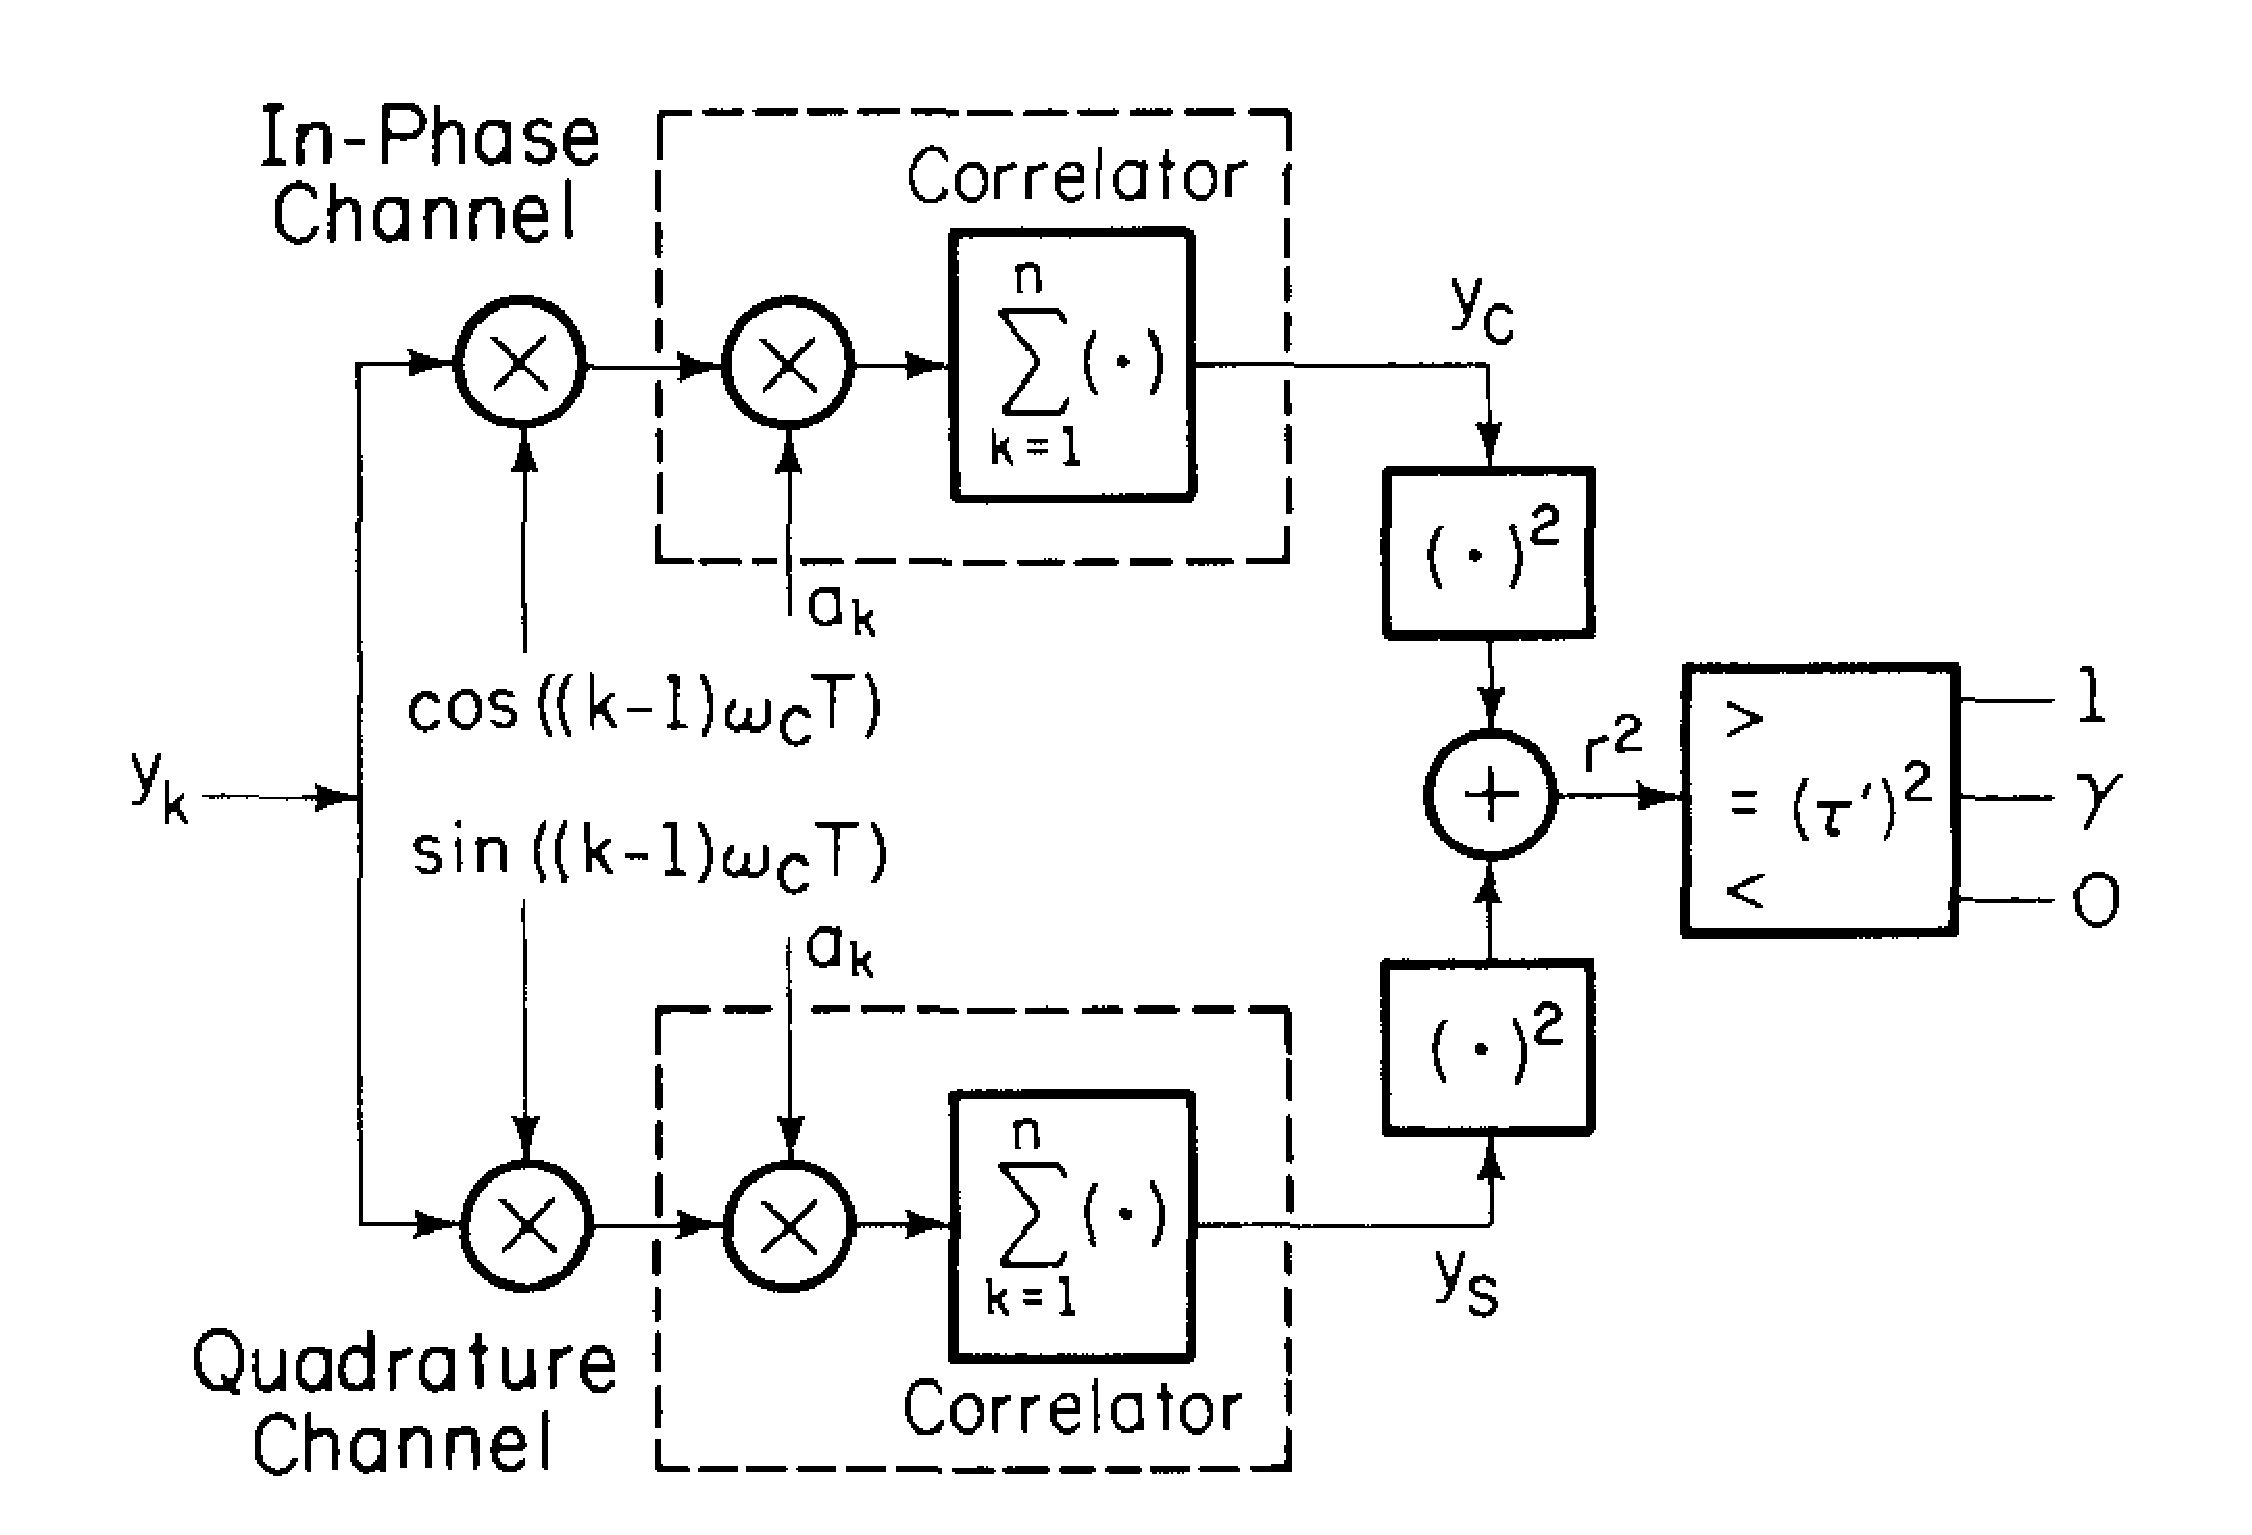
\includegraphics[scale=0.3]{Figures/Noncoherent_Detector.eps}
		\caption{Optimum system for noncoherent detection of a modulated sinusoid in i.i.d. Gaussian noise.}
		\label{fig:nonCohDetector}
	\end{figure}

	\section{Performance Analysis of the Noncoherent Detector}
	To analyze the performance of the noncoherent detector derived in the previous section, we need to compute the false alarm and detection probabilities $P_0(\Gamma_1)$ 
	and $P_1(\Gamma_1)$ respectively, where $\Gamma_1$ is the acceptance region of the noncoherent detector. The probabilities $P_0(\Gamma_1)$ and $P_1(\Gamma_1)$ are given by
	\begin{align}
	 P_j\left(\Gamma_1\right) = P_j\left(R > \tau'\right) = P_j\left(R^2 > \left(\tau'\right)^2\right),\quad j = 0, 1.
	\end{align}
	where $R = \sqrt{Y_c^2 + Y_s^2}$. Since $R$ is a function of $Y_c$ and $Y_s$, the desired probabilities can be found from the joint probability density function of 
	$Y_c$ and $Y_s$ under the hypotheses $\mathcal{H}_0$ and $\mathcal{H}_1$. For the convenience of the reader, we define $Y_c$ and $Y_s$ again below.
	\begin{align}
	\begin{aligned}
	 Y_c &\triangleq \sum_{k=1}^n a_k Y_k \cos\left[\left(k-1\right) \omega_c T_s\right]\\
	 Y_s &\triangleq \sum_{k=1}^n a_k Y_k \sin\left[\left(k-1\right) \omega_c T_s\right]
	 \end{aligned}
	\end{align}
	\subsection{Computation of probability of false alarm}
	Under $\mathcal{H}_0$, $\underline{Y}$ is $\mathcal{N}(0, \sigma^2\textbf{I}_n)$, and since $Y_c$ and $Y_s$ are linear in $\underline{Y}$, we can calculate the mean 
	and variance of $Y_c$ and $Y_s$ as follows:
	\begin{align}
	 \mathbb{E}\left\{Y_c | \mathcal{H}_0\right\} = \mathbb{E}\left\{Y_s | \mathcal{H}_0\right\} = 0.
	\end{align}
	\begin{align}
	 \text{Var}\left[Y_c | \mathcal{H}_0\right] = &\mathbb{E}\left\{Y_c^2 | \mathcal{H}_0\right\} = \sum_{k=1}^n \sum_{l=1}^n a_k a_l \mathbb{E}\left\{N_k N_l\right\}\nonumber\\
	 & \times \cos\left[\left(k-1\right)\omega_c T_s\right] \cos\left[\left(l-1\right)\omega_c T_s\right] \nonumber\\
	 = &\sigma^2 \sum_{k=1}^n a_k^2 \cos^2\left[\left(k-1\right)\omega_c T_s\right] = \frac{n\sigma^2 \overline{a^2}}{2}
	\end{align}
	where we have used the assumption in \eqref{sec_para}. Similarly, $\text{Var}\left[Y_s | \mathcal{H}_0\right]$ can also be computed to be equal to $\frac{n\sigma^2 \overline{a^2}}{2}$.
	The covariance of $Y_c$ and $Y_s$ under $\mathcal{H}_0 $ is
	\begin{align}
	 \text{Cov}\left(Y_c, Y_s | \mathcal{H}_0\right) &= \mathbb{E}\left\{Y_c Y_s | \mathcal{H}_0\right\} \nonumber\\
	 &= \sum_{k=1}^n \sum_{l=1}^n a_k a_l \cos\left[\left(k-1\right)\omega_c T_s\right] \sin\left[\left(l-1\right)\omega_c T_s\right] \nonumber\\
	 &= \frac{\sigma^2}{2} \sum_{k=1}^n a_k^2 \sin\left[2\left(k-1\right) \omega_c T_s\right] = 0.
	\end{align}
	Since $Y_c$ and $Y_s$ are jointly Gaussian and uncorrelated, they are also independent. The joint density of $Y_c$ and $Y_s$ under $\mathcal{H}_0$ is given as
	\begin{align}
	 p_{Y_c, Y_s}\left(y_c, y_s | \mathcal{H}_0\right) = \frac{1}{\pi n \sigma^2 \overline{a^2}} \text{exp}{\left\{-\frac{y_c^2 + y_s^2}{n\sigma^2\overline{a^2}}\right\}} \label{jpdfYcYs_H0}
	\end{align}
	The false alarm probability is thus given by
	\begin{align}
	 P_F(\tilde{\delta}_0) = P_0\left(\Gamma_1\right) &= \iint\limits_{\{y_c^2 + y_s^2 \ge (\tau')^2\}} p_{Y_c, Y_s}\left(y_c, y_s | \mathcal{H}_0\right) dy_c dy_s \nonumber\\
	 &= \frac{1}{\pi n \sigma^2 \overline{a^2}} \int\limits_{0}^{2 \pi} \int\limits_{\tau'}^{\infty} \text{exp}\left(-\frac{r^2}{n \sigma^2 \overline{a^2}}\right) rdr d\psi \nonumber\\
	 &= \text{exp}\left(-\frac{(\tau')^2}{n \sigma^2 \overline{a^2}}\right), \label{FalseAlarmProb}
	\end{align}
	where we used cartesian polar coordinates transformation to solve the integral.
       
	\subsection{Computation of probability of detection}
	The joint density of $Y_c$ and $Y_s$ needs to be computed under $\mathcal{H}_1$ to find the probability of detection. Given the parameter $\Theta = \theta$, $\underline{Y}$
	has a conditional distribution $\mathcal{N}(\underbar{s}(\theta), \sigma^2 \textbf{I}_n)$ under $\mathcal{H}_1$. Since $Y_c$ and $Y_s$ are linear in $\underline{Y}$ as mentioned
	earlier, they also follow a Gaussian distribution given $\Theta = \theta$. The statistics of $Y_c$ and $Y_s$ under $\mathcal{H}_1$ are calculated as below:
	\begin{align}
	 \mathbb{E}\left\{Y_c | \mathcal{H}_1, \Theta = \theta\right\} &= \sum_{k=1}^n a_k \mathbb{E}\left\{Y_k | \mathcal{H}_1, \Theta = \theta\right\} \cos\left[\left(k-1\right)\omega_c T_s\right]\nonumber\\
	 &= \sum_{k=1}^n a_k^2 \sin\left[\left(k-1\right)\omega_c T_s + \theta\right] \cos\left[\left(k-1\right)\omega_c T_s\right]\nonumber\\
	 &= \frac{n \overline{a^2}}{2} \sin\theta,
	\end{align}
	and similarly, $\mathbb{E}\left\{Y_c | \mathcal{H}_1, \Theta = \theta\right\} = \frac{n \overline{a^2}}{2} \cos\theta$. Given $\Theta = \theta$, the variances and
	covariance of $Y_c$ and $Y_s$ under $\mathcal{H}_1$ are same as that of their values under $\mathcal{H}_0$, since the only change in $\underline{Y}$ is a shift in mean.\\
	The unconditional density of $Y_c$, $Y_s$ under $\mathcal{H}_1$ is found by averaging the conditional density over $\theta$, which is given below.
	\begin{align}
	 p_{Y_c, Y_s}\left(y_c, y_s | \mathcal{H}_1\right) &= \frac{1}{2\pi} \bigint\limits_{0}^{2\pi} \frac{1}{\pi n \sigma^2 \overline{a^2}} \text{exp}{\left\{-\frac{\left(y_c - \frac{n \overline{a^2}}{2} \sin\theta\right)^2 + \left(y_s - \frac{n \overline{a^2}}{2} \cos\theta\right)^2}{n\sigma^2\overline{a^2}}\right\}} d\theta\nonumber\\
	 &= p_{Y_c, Y_s}\left(y_c, y_s | \mathcal{H}_0\right) \text{exp}\left\{-\frac{n \overline{a^2}}{4\sigma^2}\right\} I_0\left(\frac{\left[y_c^2+y_s^2\right]^\frac12}{\sigma^2}\right),
	\end{align}
	where $I_0$ is the zeroth order modified Bessel function of the first kind. The detection probability thus becomes
	\begin{align}
	 P_D(\tilde{\delta}_0) = P_1\left(\Gamma_1\right) &= \iint\limits_{\{y_c^2 + y_s^2 \ge (\tau')^2\}} p_{Y_c, Y_s}\left(y_c, y_s | \mathcal{H}_1\right) dy_c dy_s \nonumber\\
	 &= \frac{e^{-\frac{n\overline{a^2}}{4\sigma^2}}}{\pi n \sigma^2 \overline{a^2}} \int\limits_0^{2\pi} \int\limits_{\tau'}^{\infty}r \text{exp}\left\{-\frac{r^2}{n \sigma^2 \overline{a^2}}\right\} I_0\left(\frac{r}{\sigma^2}\right) dr d\psi \nonumber\\
	 &= \int\limits_{\tau_0}^{\infty} x \text{exp}\left\{-\frac{x^2+b^2}{2}\right\} I_0\left(bx\right)dx \triangleq Q\left(b, \tau_0\right), \label{MarcQfunc}
	\end{align}
	where $b^2 \triangleq \frac{n\overline{a^2}}{2\sigma^2}$ and $\tau_0 \triangleq \frac{\tau'}{\sigma^2 b}$. We have made the substitution $x = \frac{r}{\sigma^2 b}$ in the above integral.
	The function $Q$ in \eqref{MarcQfunc} is sometimes known as \textit{Marcum's Q-function}.\\
	From \eqref{FalseAlarmProb}, we can set the threshold for $\alpha$-level Neyman-Pearson detection in this problem. We get the threshold as
	\begin{align}
	 \tau' = \left[n \sigma^2 \overline{a^2}\operatorname*{log}\left(\frac{1}{\alpha}\right)\right]^\frac12.
	\end{align}
	For this threshold, the detection probability can be calculated as
	\begin{align}
	 P_D(\tilde{\delta}_0) = Q\left(b, \left[2 \operatorname*{log}\left(\frac{1}{\alpha}\right)\right]^\frac12\right).
	\end{align}
	The average signal energy is
	\begin{align}
	 \mathbb{E}\left\{\frac{1}{n}\sum_{k=1}^n s_k^2(\Theta)\right\} = \frac{1}{n} \frac{1}{2\pi} \int\limits_0^{2\pi} \sum_{k=1}^n a_k^2 \sin^2\left[\left(k-1\right)\omega_c T_s + \theta\right] d\theta = \frac{\overline{a^2}}{2}.
	\end{align}
	Thus $b^2 = \frac{n \overline{a^2}}{2 \sigma^2}$ can be interpreted as signal-to-noise ratio of the noncoherent detector. For a coherent detector, the corresponding
	value of SNR would be
	\begin{align}
	 d^2 = \frac{1}{\sigma^2} \sum_{k=1}^n s_k^2\left(\theta\right) = \frac{n \overline{a^2}}{2\sigma^2} = b^2.
	\end{align}
	For the range of SNR and $\alpha$ occuring in most practical problems, we have
	\begin{align}
	 Q\left(b, \left[2 \operatorname*{log}\left(\frac{1}{\alpha}\right)\right]^\frac12\right) = 1 - \Phi\left[\Phi^{-1}\left(1-\alpha\right) - d\right],
	\end{align}
	when $b = d + 0.4$.\\
	The disadvantage with noncoherent detector is that, the performance for fixed $\alpha$ is inferior when compared to a coherent detector with $b = d$. So,
	a higher SNR is required for a noncoherent detector to meet the performance of a coherent detector.
	However, a noncoherent	detector does not need to have the knowledge of carrier phase, whereas a coherent detector needs carrier phase tracking system to 
	synchronize the phases of the transmitter and receiver.


	
\end{document}